
\section{The Calm Before the Storm}

\subsection{Checks, Balances, and Blind Spots}

David signed it.

A single initial. Black ink on cream bond paper.
The final signature on a memo that had already made its way through Risk, Compliance, and Ops.

He set the pen down and exhaled — not relief, just movement.

\medskip

\begin{figure}[H]
  \centering
  \begin{tikzpicture}[
    node distance=1.8cm and 3cm,
    every node/.style={draw, rounded corners, minimum width=3cm, minimum height=1.5cm, align=center},
    arrow/.style={->, thick}
  ]

    % Nodes
    \node (risk) {Risk\\\small Evaluates exposure\\and model behavior};
    \node (compliance) [right=of risk] {Compliance\\\small Checks mandate\\alignment};
    \node (ops) [right=of compliance] {Ops\\\small Ensures systems,\\routing, execution};
    \node (memo) [below=of compliance] {Memo\\\small Phase II Expansion Approval};
    \node (david) [below=of memo] {David\\\small Final Sign-off};

    % Arrows
    \draw[arrow] (risk) -- (memo);
    \draw[arrow] (compliance) -- (memo);
    \draw[arrow] (ops) -- (memo);
    \draw[arrow] (memo) -- (david);

  \end{tikzpicture}
  \caption{Approval Flow for Phase II Expansion: Risk, Compliance, and Ops all feed into a shared memo reviewed 
  and signed by David.}
\end{figure}

\medskip

\begin{HistoricalSidebar}{Checks and Balances: From Philosophy to Policy}

  The idea of \textbf{checks and balances} — that no single branch or actor should hold unchecked power — traces its 
  roots to the 18th-century political philosopher \textbf{Montesquieu}. In his seminal work, \textit{The Spirit of the 
  Laws} (1748), Montesquieu argued that liberty could only be preserved if power was divided among distinct branches 
  of government: \textit{legislative}, \textit{executive}, and \textit{judicial}. Each branch, he claimed, must be 
  both independent and able to restrain the others.
  
  This principle deeply influenced the \textbf{Founding Fathers of the United States}. Drawing on Montesquieu’s insights, 
  they embedded a system of checks and balances into the U.S. Constitution. Congress could make laws, but the President 
  could veto them. The judiciary could interpret laws, but judges were appointed by the President and confirmed by the 
  Senate. Power, in this design, was fragmented — not to create gridlock, but to force accountability.
  
  \medskip
  
  In modern institutional design --- from financial firms to AI governance --- echoes of this philosophy remain. When it works, 
  no one can act unilaterally. When it fails, it’s often not from the absence of rules, but from the erosion of enforcement, 
  transparency, or communication across those “separate” branches.
  
\end{HistoricalSidebar}

\medskip

The initial run had been a triumph.

Aurora’s Q1 strategy — a volatility-harvest framework with adaptive rebalancing — had done more than 
outperform. It had delivered something far rarer: uncorrelated alpha that actually held.

\medskip

\begin{TechnicalSidebar}{What is Uncorrelated Alpha?}

  In finance, \textbf{alpha} refers to the portion of an investment’s return that exceeds a benchmark — a measure of 
  “skill-based” performance, not just market movement. But not all alpha is created equal.
  
  \medskip
  
  \textbf{Uncorrelated alpha} is the holy grail: returns that are both \textit{above benchmark} and \textit{independent} 
  of broader market swings. This means the strategy isn't just riding a bull market — it’s generating value regardless 
  of whether the S\&P rises or falls.
  
  \medskip
  
  Why does this matter?

  \medskip
  
  \begin{itemize}
    \item For multi-strategy funds and institutional allocators, uncorrelated alpha provides \textbf{diversification 
    at the return level}, not just the asset level.
    \item It helps smooth out portfolio volatility and reduce exposure to systemic risk.
    \item In regulatory or capital-constrained environments, it improves \textbf{risk-adjusted performance without 
    increasing gross exposure}.
  \end{itemize}
  
  \medskip
  
  In Aurora’s case, the Q1 strategy delivered alpha that held steady even as major asset classes whipsawed — not because 
  it avoided volatility, but because it \textit{harvested} it in ways other models couldn't track. That’s what made 
  it valuable.
  
\end{TechnicalSidebar}

\medskip


Tight spreads.
Low drawdown.
Nearly half a billion in net gains — clean.

It wasn’t just the money. It was the elegance.
The model moved like a scalpel — slicing volatility, balancing exposure, skating between rails others hadn’t even mapped.

“Four-eighty,” the board had repeated, almost reverently, at the last performance review.
And with it came the question that wasn’t a question:
\textit{If it works here, can it scale across jurisdictions?}

David had hesitated — not out loud, but inside.
The timing felt wrong. The sync issues were still unresolved. Regulatory variance made synthetic exposure a minefield.

But Hart had leaned in, all charm and conviction.
“This isn’t just performance,” he’d said. “It’s a narrative. Aurora’s running headlines. Investors love velocity.”

And it was true — they were moving fast.
Too fast for David’s comfort.
But somehow, impossibly, they kept pulling it off.

And with it: a question that wasn’t really a question.

\textit{If it works here, can it scale across jurisdictions?}

So Phase II was approved:
\textbf{Cross-jurisdictional execution}, routed through Arcadia’s London desk.

\medskip

\begin{HistoricalSidebar}{Cross-Jurisdictional Execution: Speed, Fragmentation, and Shadows}

  Cross-jurisdictional execution — the routing of trades across international desks to exploit latency, regulatory 
  arbitrage, or access — has long been both a competitive advantage and a systemic blind spot.

  \medskip
  
  In the early 2000s, hedge funds began routing European equity trades through U.S. dark pools to avoid MiFID 
  restrictions. Conversely, U.S. desks routed through London to exploit favorable derivatives treatment. The 2010 
  Flash Crash revealed how fragmented venues, spread across time zones and compliance domains, could react with 
  incoherent logic in milliseconds.

  \medskip
  
  By 2015, major asset managers were running execution algorithms that spanned Tokyo, London, Frankfurt, and New 
  York — often with asynchronous oversight. Compliance regimes couldn’t keep up.

  \medskip
  
  Cross-border desks brought speed and flexibility — especially in synthetic instruments like CFDs, TRSs, and 
  offshore swaps. But they also brought latency mismatches, disconnected kill switches, and jurisdictional confusion 
  in crisis response.

  \medskip
  
  After Archegos (2021), regulators flagged how synthetic positions spread across prime brokers in different legal 
  systems could accumulate unmonitored. But enforcement lagged.

  \medskip
  
  \textbf{The promise:} optimal routing, alpha capture, and 24/6 liquidity.

  \medskip

  \textbf{The risk:} fragmented oversight, circular hedging, and response delays measured in billions.
  
\end{HistoricalSidebar}

\medskip



\subsection{Elastic Exposure, Rigid Assumptions}

The pitch was simple:
Tighter latency on European venues.
Flexible regulatory treatment of synthetic instruments.
Speed, at scale.

The risk?
\textit{Contained.} At least according to the memo.

David glanced at the terminal again.

“London live?” he asked.

Kayla tapped her screen. “Ten minutes ago. No anomalies. Feeds are clean.”

He gave a shallow nod.

“Keep it tight,” he said. “No experimentation on deployment night.”

“Understood,” she replied, already turning.

David remained still for a moment.

The floor buzzed on.

No alarm.
No warning.

Just another initial.
Another memo.
And a strategy that had never known a storm.


He didn’t love the language.

\textit{“Elastic notional synthesis.” “Latency-sliced positioning.” “Behavior-aware hedging.”}

It read like a PowerPoint built for people who liked the sound of algorithms more than the feel of them.

But it wasn’t his call anymore.

David had scoped the model with his team — built it to breathe in narrow bands, calibrated for edge 
cases and gentle undulations.
It wasn’t built for speed.
It was built for resilience.

\medskip

\begin{TechnicalSidebar}{Why Machine Learning Models Must Be Continuously Trained}

  Machine learning models are not static assets.  
  They are probabilistic approximators—trained not to be \textit{correct}, but to be \textit{informationally relevant} to the distribution they’ve seen.
  
  \medskip
  
  \textbf{But that distribution moves.}

  \medskip
  
  In trading systems, this is called \textit{non-stationarity}. In ML theory, it's \textit{distributional drift}. In practical terms:  
  what worked yesterday might fail quietly tomorrow.
  
  \medskip
  
  A model trained on old market conditions may:

  \medskip
  
  \begin{itemize}
    \item Suppress signals it now considers noise
    \item Misclassify valid anomalies as benign
    \item Overfit to structural patterns that no longer exist
  \end{itemize}

  \medskip
  
  Worse: without retraining, the confidence scores remain high—even as accuracy degrades.  
  This is the most dangerous form of model failure: \textbf{not silent, but self-assured.}
  
  \medskip
  
  \textbf{Continuous retraining} isn’t a nice-to-have. It’s survival.  

  \medskip

  It requires:

  \medskip
  
  \begin{itemize}
    \item Streaming pipelines for ingesting new data
    \item Validation infrastructure that can reweight on the fly
    \item Human oversight for flagging edge-case drift before it calcifies into error
  \end{itemize}

  \medskip
  
  In theory, all models degrade.  
  In practice, only the ones that get updated stay useful.
  
\end{TechnicalSidebar}

\medskip

\begin{HistoricalSidebar}{The Zillow Collapse}

  \textbf{In 2021, Zillow learned the hard way what happens when a model goes stale.}

  \medskip
  
  At the heart of its failure was the \textit{Zestimate} algorithm—a proprietary machine learning model built to 
  predict home values.  
  Zillow wasn't just using it for browsing anymore. They were using it to buy real houses.
  
  \medskip
  
  \textbf{The bet:} if their model was accurate within a narrow margin, they could algorithmically flip properties at scale.  

  \medskip

  \textbf{The reality:} the model was trained on historical data, in a market that was changing faster than the 
  retraining loop could adapt.
  
  \medskip
  
  \textbf{What went wrong?}

  \medskip
  
  \begin{itemize}
    \item \textbf{Feedback lag:} The model relied on past sale data. But in a hot market, sale prices lagged real-time 
    demand shifts.
    \item \textbf{Distributional drift:} Market dynamics changed post-COVID—inventory shocks, urban flight, remote 
    work—but the model assumed stationarity.
    \item \textbf{Overconfidence:} As model performance degraded, Zillow continued scaling up purchases—trusting 
    predictions that no longer reflected reality.
  \end{itemize}

  \medskip
  
  \textbf{The result:}  Zillow wrote down over \$500 million in losses, liquidated its inventory, and laid off 25\% of 
  its workforce.
  
  \medskip
  
  The lesson wasn’t just about real estate.  
  It was about models—and what happens when leadership mistakes \textit{confidence} for \textit{validity}.
  
  Zillow didn’t just misprice homes.  
  They operationalized a model faster than they could audit it.
  
  And the market noticed.
  
\end{HistoricalSidebar}

\medskip

\begin{figure}[H]
  \centering
  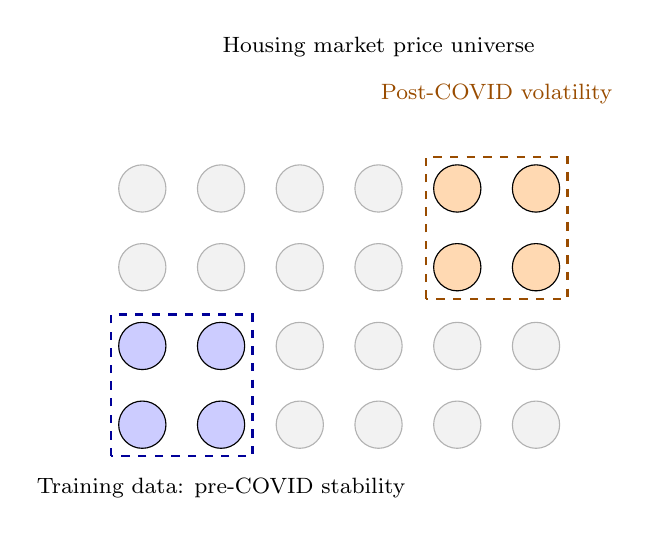
\begin{tikzpicture}[
      stable/.style={circle, draw=black, fill=blue!20, minimum size=0.6cm},
      covid/.style={circle, draw=black, fill=orange!30, minimum size=0.6cm},
      neutral/.style={circle, draw=black!30, fill=gray!10, minimum size=0.6cm},
      every node/.style={font=\scriptsize}
  ]
  
  % Grid layout (6x4)
  \foreach \x in {0,1,2,3,4,5} {
      \foreach \y in {0,1,2,3} {
          \node[neutral] (n\x\y) at (\x, \y) {};
      }
  }

  % Training data for stable market (left 2x2)
  \foreach \x in {0,1} {
      \foreach \y in {0,1} {
          \node[stable] at (\x, \y) {};
      }
  }

  % New dynamics during COVID (right 2x2)
  \foreach \x in {4,5} {
      \foreach \y in {2,3} {
          \node[covid] at (\x, \y) {};
      }
  }

  % Labels
  \node[align=left, font=\footnotesize] at (1, -0.8) {Training data: pre-COVID stability};
  \node[align=left, font=\footnotesize, text=orange!60!black] at (4.5, 4.2) {Post-COVID volatility};
  \node[align=left, font=\footnotesize] at (3, 4.8) {Housing market price universe};

  \draw[dashed, thick, blue!60!black] (-0.4, -0.4) rectangle (1.4, 1.4);
  \draw[dashed, thick, orange!60!black] (3.6, 1.6) rectangle (5.4, 3.4);

  \end{tikzpicture}
  \caption{Model Failure from Distributional Drift: Zillow’s prediction engine trained on pre-COVID stability (blue), but volatility emerged in unmodeled housing zones (orange).}
\end{figure}


  



Then Hart got involved.
Then the deck changed.
Then Arcadia routed it through London.

It launched clean.

No glitches. No unexpected slippage.
Just the quiet hum of code doing what it was told.

For 48 hours, it was flawless.

Small trades.
Tight deltas.
Mostly commodities
\footnote{\textbf{Commodities} are raw physical goods like oil, natural gas, gold, wheat, and copper that are traded 
on markets. Unlike stocks or bonds, commodities are standardized, interchangeable assets typically bought and sold via 
futures contracts. Traders often use commodities to hedge against inflation, geopolitical risk, or supply chain 
disruptions.}
and volatility hedges, 
\footnote{\textbf{Volatility hedges} are financial strategies or instruments used to protect a portfolio from sharp market 
swings. Instead of betting on price direction, they aim to profit when market uncertainty increases — often using options, 
variance swaps, or VIX-linked products. These hedges act like insurance against turbulence.}
running hot but steady — all green.

David watched it from the second screen at Arcadia’s control room, seated off-center from the main pit.
He didn’t hover.
He observed.

No alerts. No errors.
Just numbers, printing in calm rhythm.

\subsection{The Architecture of Execution}

Across the floor, terminals glowed in muted hues.  The espresso machine hissed like a stress valve.  It was morning in 
New York, and London was already deep into the session.

Kayla, from execution strategy, leaned in through the open doorframe.

\medskip

\begin{TechnicalSidebar}{What Is Execution Strategy?}

  \textbf{Execution strategy} is the set of methods, rules, and tools used to convert a trading idea into actual trades — 
  as efficiently and cost-effectively as possible.
  
  \medskip
  
  In modern markets, the challenge isn’t just \textit{what} to buy or sell. It’s \textit{how}.
  
  \medskip
  
  An execution strategist focuses on:
  
  \begin{itemize}
    \item \textbf{Minimizing slippage:} ensuring trades don’t move the market too much.
    \item \textbf{Timing and fragmentation:} deciding which venues to hit, in what sequence, and at what speed.
    \item \textbf{Adaptive routing:} choosing real-time paths through exchanges, dark pools, and synthetic liquidity 
    providers.
    \item \textbf{Managing execution risk:} monitoring fills, latency, and adverse selection.
  \end{itemize}
  
  \medskip
  
  At the institutional level, execution strategy blends quantitative modeling with market microstructure expertise 
  because even a perfect model can underperform if executed poorly.
  
\end{TechnicalSidebar}

\medskip

“London’s cleared for rollout,” she said, stopping a few feet behind him. “I verified that we’re pre-positioned 
across the LSE, Cboe Europe, and Turquoise venues.”

\medskip

\begin{TechnicalSidebar}{What is Pre-Positioning?}

  \textbf{Pre-positioning} refers to the strategic placement of capital, orders, or algorithmic models across multiple 
  trading venues \textit{before} execution begins.  
  It ensures that when the market moves — or when a system is triggered — the infrastructure is already in place to 
  respond instantly.

  \medskip

  In high-frequency or cross-jurisdictional trading, milliseconds matter.  
  Pre-positioning reduces latency and slippage by eliminating the need to request access or deploy logic in real time.

  \medskip

  It can include:

  \begin{itemize}
    \item \textbf{Capital allocation:} Ensuring margin or collateral is already posted at multiple exchanges.
    \item \textbf{Order scaffolding:} Pre-loaded orders or algorithms waiting for live market triggers.
    \item \textbf{Model mirroring:} Synchronizing trading models across geographies (e.g., New York, London, Singapore) 
    for rapid parallel execution.
    \item \textbf{Infrastructure warm-up:} Keeping compute resources active and primed to route orders.
  \end{itemize}

  \medskip

  In Kayla’s update, “pre-positioned across three venues” means Aurora’s systems had already staged trades and routing 
  logic in advance.  
  The model could engage immediately — no warm-up, no requests, just execution. It’s how you move fast in markets that 
  punish hesitation.

\end{TechnicalSidebar}

\medskip

David didn’t turn around. He just nodded — a nod that said yes, but thought God, I hope so.

Because even now, even after the test clears and the checklist ticks, the reel is still playing in his head — 
back to the room where they’d made the call.

They’d been in Geneva, two weeks before rollout. A whiteboard full of venue maps, latency curves, and fill 
curves was still half-visible behind the reflection of the window.

"Three tiers?" someone had asked.
"No. We pick three names we trust," David had said.
"LSE, Cboe Europe, Turquoise. Between them, you cover core liquidity, synthetic rerouting, and dark overlays."

"But we could split across eight—"
"—and get eight different risk profiles," he’d cut in.

He remembered tapping the board with the back of his pen.
“We’re not building an experiment. We’re building a highway.”

He remembered thinking: venues are like roads.
You don’t just care if they’re open. You care what kind of traffic they carry.

\begin{itemize}
\item \textbf{LSE} was legacy. Deep books, predictable behavior, slower to stress. Like a stable old artery through the city.
\item \textbf{Cboe Europe} had agility — tighter spreads, cross-product hooks, and better slippage handling in high-turnover names.
\item \textbf{Turquoise} was the wildcard: low visibility, better dark fill ratios, optional midpoint matching.
\end{itemize}

Each venue was its own ecosystem — its own style of liquidity.
They weren’t just execution pipes. They were behavioral signatures.

And choosing them meant choosing the kind of failure you were willing to have.

Back then, he had said it out loud:
"If it breaks, I’d rather break predictably. I’d rather break where I know who else is in the water."

Now, standing at the desk, he wished he’d spent more time modeling what happened when they all broke the same way.

He could still hear his own voice from Geneva, calm and confident:
\textit{"We’re not building an experiment."}

But now, watching the screen, that’s exactly what it felt like.

An experiment they couldn’t rewind.
And a test that wasn’t finished until it failed.

\subsection{Staggered Ignition}

David didn’t turn. “All equity, as expected?”

“Cash and ETF blocks only,” she confirmed. “Derivs stay in Chicago, FX still sleeps until New York opens. 
Core inventory’s clean and loaded.”

He gave a fractional nod — one that looked like acceptance but felt like interrogation.

Because in his head, the clock wound backward again — to the allocation meetings.
To the diagrams.
To the models they thought were conservative enough.

\textit{That meeting had happened in a glass-walled room with the clocks muted.}

They’d gone line by line through the flowbook.

“Cash leads?”
“Yes — equities first. Faster to price. Easier to throttle.”

“And ETFs?”
“They’re shallow pre-open but safer than futures. No mark-to-market shock if we get slippage.”

“Derivs?”
“Hold them. Vol’s still gapped. Chicago has latency advantage, and we don’t want hedges waking up before the hedge need exists.”

“FX?”
“Asleep until 08:00 New York. Let it stay asleep.”

They had built the book with military logic — not for speed, but for order.

The thesis was: \textbf{staggered ignition.}

\begin{itemize}
\item \textbf{Cash equity first}, for clarity and control.
\item \textbf{ETF blocks} second, to scale without drawing attention.
\item \textbf{Derivatives deferred}, to avoid triggering the machines.
\item \textbf{FX last}, because currency would follow — not lead — the story.
\end{itemize}

David had stood at the board, drawing concentric rings like a launch sequence.

\textit{“We don’t launch a platform,” he’d said. “We light a fuse.”}

Now, standing at the desk with the screen glowing faintly against the silence,
he wondered if they had timed the sequence wrong.
If they had front-loaded clarity — but back-loaded defense.
If they had planned for containment — but not for inversion.

He didn’t turn.
Didn’t blink.
Just replayed the fuse again, from the spark.




\subsection{Split Personality Execution}

He nodded faintly, eyes on the skyline. “And the styles?”

“Turquoise for size, low impact,” she said, without hesitation. “Cboe to edge the lit with minimal footprint. 
LSE anchors the open which is still the best for cross-border legs.”

“Lit and dark mix still holding?”

“Split personality intact,” she said, almost smiling. “We haven’t rebalanced the blend. At least, not 
until we see venue behavior stabilize.”

“And we’re matching order types to venue behavior?”

“Midpoint pegs on Turquoise,” she said. “Post-only on Cboe. Adaptive VWAP on LSE. Strategy’s still 
context-driven.”

David didn’t respond. Not immediately.

Because in his head, he was already back in Basel —
the room with too many chairs, a screen too small for the number of opinions,
and a whiteboard divided vertically between \textit{lit} and \textit{dark}.

\textit{It had been about styles, yes. But more than that, it was about behavior.
What the venue \textbf{said} it was — and what it actually did under pressure.}

“Turquoise is dark, but not invisible,” one quant had said.
“Exactly,” David replied. “We want size without signaling. Midpoint peg only. If it moves, we’re too visible.”

“Cboe?”
“Cboe’s the knife,” someone had said. “Edge, don’t slash.”

They had nodded. Cboe would be for precision — post-only, lit but limited.
The goal: extract without leaving footprints.

“LSE?”
“Still the benchmark,” David had said. “Use it to anchor. VWAP logic. Let it signal confidence in the open.”

And then someone else — risk, probably — had asked:
“Do we trust the mix? Lit versus dark? Cross-referenced flow?”

David had drawn a line down the board and said:
\textit{“We don’t want a personality. We want a split personality.”}

That had gotten a laugh. But it wasn’t a joke.

It was the entire thesis: balance the visible with the hidden.
Use each venue for what it claims to be — until it stops behaving that way.

\textbf{Context-driven strategy.}
Execution styles shaped not just by cost — but by venue psychology.

They had built a system that watched how each venue behaved
and adjusted the order types accordingly.
Not static — adaptive. Behavioral matching at microstructure speed.

\textit{At least, that was the idea.}

Now, standing in silence above the London skyline,
he wondered if the behavior had changed underneath them.
If the venues were still who they said they were.
If the “personality split” had become a personality disorder.

He didn’t ask.
Because asking would mean they weren’t sure.
And right now, uncertainty was still the most expensive order type in the book.

% Add vertical padding to table rows
\renewcommand{\arraystretch}{1.4}  % Adjust this value for more or less padding

\begin{table}[H]
\centering
\rowcolors{2}{gray!10}{white}
\resizebox{\textwidth}{!}{%
\begin{tabular}{
  >{\raggedright\arraybackslash}p{2.5cm} 
  >{\raggedright\arraybackslash}p{2.8cm} 
  >{\raggedright\arraybackslash}p{4.3cm} 
  >{\raggedright\arraybackslash}p{5.2cm}
}
\toprule
\textbf{Venue} & \textbf{Style} & \textbf{Behavior} & \textbf{Risk} \\
\midrule
Turquoise & Midpoint Peg & Stealth, Low Impact & \faExclamationTriangle\quad Crowding, Signal Leakage \\
Cboe Europe & Post-Only & Edge Probing, Low Footprint & \faBomb\quad Spoof Sensitivity, Slippage \\
LSE & Adaptive VWAP & Visible Intent, Benchmarked & \faExclamationCircle\quad Market Impact, Front-Run Risk \\
\bottomrule
\end{tabular}%
}
\caption{Mapping of Venues to Execution Styles, Behaviors, and Risk Profiles}
\end{table}
  


\begin{TechnicalSidebar}{Venue Psychology and Execution Style}

  Modern execution strategy isn't just about spreads, fees, or latency.  
  It's about understanding \textbf{venue psychology} — how different trading venues behave under different conditions — and aligning order styles to match.

  \medskip

  Each venue has a \textit{personality}:
  \begin{itemize}
    \item Some venues reward size and patience.
    \item Others reward speed, precision, and timing.
    \item Some appear liquid but evaporate under stress.
    \item Others stay shallow — but stable.
  \end{itemize}

  \medskip

  \textbf{Execution styles} must be mapped to these traits:

  \begin{itemize}
    \item \textbf{Turquoise (dark pool):} 
    Use \textit{midpoint pegs} to extract large blocks without signaling.  
    Treat it as low-impact, but visibility-sensitive. Good for size, risky if crowded.

    \item \textbf{Cboe Europe (lit venue):} 
    Use \textit{post-only} to lightly probe liquidity without triggering reactions.  
    Designed for tactical presence — extract edge without chasing fills.

    \item \textbf{LSE (anchor venue):} 
    Use \textit{adaptive VWAP} to participate gradually across the open, especially for cross-border flows.  
    Best for establishing visible intent without overcommitting early.

  \end{itemize}

  \medskip

  \textbf{Why it matters:}

  Sending the wrong order type to the wrong venue is like wearing a tuxedo to a street fight — you'll look right, but you’ll bleed anyway.

  \medskip

  When venue behavior shifts — due to volatility, crowding, or regime change — execution logic must adapt.  
  That’s why strategy isn’t static. It’s \textit{context-driven}, behavior-aware, and continually rebalanced.

  \medskip

  Good execution isn't just smart. It's self-aware.

\end{TechnicalSidebar}








\subsection{Waiting to Be Right}

He finally turned slightly, catching her reflection in the window glass.
“And the FX legs?”

“Still parked. Cross-asset logic isn’t tuned for New York latency. If the hedge legs fire early, we misprice the unwind.”

He gave the faintest nod.
“Chicago?”

“Still sandboxed,” she said. “The derivs desk are decoupled on their clock, and their book.”

David looked away from the window at last.
“So the framework’s stitched, but only London’s alive.”

Kayla nodded.
“We’re letting the aggregator read the book before it touches size.”

He watched her now, full-on.
“Good. Just make sure it doesn’t misread what it sees.”

But even as he said it, the words were already replaying in his mind —
not Kayla’s, but the voices from Zurich.
From the windowless ops room with a latency heatmap projected above the trading floor like a weather 
radar for execution risk.

Someone had drawn three boxes on the board: FX, Derivs, and Cash.
Underneath them, arrows. Some bold. Some dashed. Some curved like they didn’t trust causality.

David had stood at the front and said:
“This is not a relay. It’s a choreography.”

“Then why not fire FX first?” someone had asked.
“Because FX moves before we do,” he replied. “If we hedge before the primary touches, we tell the 
street what we’re about to do.”

“And derivs?”

“They live in Chicago time. If we sync their clock to London, we break their book. If we don’t, 
we break ours.”

It had been one of those sessions — the kind where no one raised their voice because everyone 
understood the cost of being wrong.

What they had built wasn’t fragile, not exactly.
But it was threaded — stitched across markets like a pressure-sensitive suit.

Touch one panel wrong, and the whole garment wrinkles.
Touch it at the wrong time, and the seams tear.

Back then, someone from compliance had asked:
\textit{“What’s the fallback if one leg gets mispriced?”}

David didn’t blink.
“There isn’t one. That’s why we wait.”

Now, back in London, looking out over the city’s metal-glass silence,
he realized what the whole plan had always been:

Wait just long enough to be right.
But not so long that the market realizes you’re late.

Because latency isn’t just delay.
Latency is a window.
And if it closes on you mid-leg,
there’s no price in the book clean enough to fix it.





\subsection{What You Could Get Away With}


David nodded without looking up. “Synthetic hedge platform ready?”

\medskip

\begin{TechnicalSidebar}{What is a Synthetic Hedge?}

  A \textbf{synthetic hedge} is a way to mimic the protective effect of a traditional hedge without holding the actual asset.  
  Instead of directly owning the asset you want to protect — like a stock or a commodity — you construct a position 
  using financial derivatives such as:

  \medskip

  \begin{itemize}
    \item \textbf{Futures} — contracts to buy/sell the asset later at a fixed price.
    \item \textbf{Options} — rights (but not obligations) to buy/sell at specific strike prices.
    \item \textbf{Swaps} — agreements to exchange cash flows tied to an asset’s performance.
  \end{itemize}

  \medskip

  These instruments allow you to \textit{replicate} exposure, neutralize risk, or generate offsetting returns — all without 
  touching the physical asset.

  \medskip

  Synthetic hedges are faster to deploy, easier to scale across jurisdictions, and often cheaper in terms of capital 
  or regulation. But they also come with trade-offs:

  \medskip

  \begin{itemize}
    \item Increased model risk — due to abstraction from underlying market mechanics.
    \item Potential for hidden leverage.
    \item Sensitivity to correlation assumptions and counterparty exposure.
  \end{itemize}

  \medskip

  In David’s case, the synthetic hedge platform meant Arcadia could rebalance across global venues without triggering 
  the same regulatory constraints — but it also meant any misalignment could propagate faster than legacy systems 
  could catch.

\end{TechnicalSidebar}

\medskip

“Yep. EU regulation’s lighter on delta thresholds. Means more elasticity on notional wraps.”

\medskip

\begin{TechnicalSidebar}{What Are Delta Thresholds?}

  In trading, \textbf{delta} measures how much the value of a position changes in response to a change in the price 
  of the underlying asset.  
  A delta of 1.0 means a \$1 move in the asset causes a \$1 move in the position. A delta of 0.5 means only a \$0.50 
  move, and so on.

  \medskip

  \textbf{Delta thresholds} are regulatory or internal risk limits that restrict how much directional exposure a 
  portfolio or synthetic instrument can carry.  
  These thresholds are especially important for complex or leveraged positions, such as:

  \medskip

  \begin{itemize}
    \item \textbf{Derivatives with embedded leverage}
    \item \textbf{Synthetic swaps or basket trades}
    \item \textbf{Algorithmically generated hedges}
  \end{itemize}

  \medskip

  Tighter delta thresholds mean tighter control — trades must stay close to neutral or hedged exposure.  
  Looser thresholds allow greater directional bets, larger notional swings, and more elasticity in how positions 
  are wrapped and deployed.

  \medskip

  In this case, EU regulation being “lighter on delta thresholds” means the model can take on more delta — more 
  market sensitivity —  
  without triggering a compliance block. It creates flexibility, but also introduces risk: the system can swing 
  wider before hitting a stop.

\end{TechnicalSidebar}

\medskip

The words that landed were clean, confident, and factual.
But in his mind, they echoed with the ghost of a whiteboard marker squeaking on glass.

He was back in Luxembourg.

Not the conference room — the smaller one. The off-calendar prep call before the vendor roadshow.
Where the conversation hadn’t been about compliance. It had been about \textit{what you could get away with, if the delta didn’t spike}.

\textit{“We wrap it tight — low delta, small notional, but levered exposure.”}
That had been Sofia from structuring. Calm, like she was describing the weather.

“Don’t we need swap disclosure?” someone had asked.

\textit{“Not if the exposure stays within bounds.”}

David had stared at the model on screen.
An options tree with synthetic deltas shaded like heat zones.

He had asked:
“What's the elasticity look like under stress?”

Sofia:
\textit{“Better than real. Because we’re modeling control, not cash.”}

Someone else:
\textit{“If real hedges cost too much, synthetics give you a pass.”}

David remembered the way that felt. Not wrong — just fast.
A feeling that the trade wasn't being made. It was being described into existence.

He had said yes. Eventually.
Because when the desk asked for exposure without visibility,
synthetics were the answer that didn’t have to be explained in the audit notes —
only in the footnotes.

\medskip

Back in London now, he stared out over the skyline,
remembering how they’d phrased it:
\textit{“EU reg lets us flex the wrap.”}

Flex. Not “hedge.” Not “protect.”
Just... flex.

And he wondered, not for the first time,
if elasticity was just another word for a loophole
you haven't been caught using yet.


“And the latency?”

“Thirty-seven milliseconds desk to desk. Aurora’s already ported the model footprint to the London grid. 
Real-time sync across venues.”

\medskip

\begin{TechnicalSidebar}{Why Latency Matters in Trading}

  \textbf{Latency} refers to the delay between the moment a trading signal is generated and when it is executed 
  on an exchange.  
  In high-frequency and cross-venue trading, even a few milliseconds can mean the difference between arbitrage 
  and loss.

  \medskip

  \textbf{Thirty-seven milliseconds desk to desk} might sound fast — but in trading terms, it’s an eternity 
  compared to sub-millisecond co-located systems.  

  \medskip

  That latency includes:

  \begin{itemize}
    \item Signal generation and transmission
    \item Routing across network hops (e.g., New York to London)
    \item Exchange confirmation and roundtrip acknowledgment
  \end{itemize}

  \medskip

  \textbf{Porting the model to the London grid} means Aurora reduced some of that latency by shifting compute 
  closer to the venue.  
  Real-time synchronization across venues ensures consistency in state — but only if latency is stable and 
  predictable.

  \medskip

  In this case, 37ms isn't just a number — it's a performance ceiling.  
  It defines how reactive the system can be under stress, and how quickly risk can be neutralized when the 
  market turns.

\end{TechnicalSidebar}

\medskip

David leaned back, eyes scanning the floor. It looked calm.
It always did right before.




